\section{Preliminary}
\label{sec:prel}


In this section we first present the generalized inference model, and then introduce our empirical observations on the relationship strengths measure.


\subsection{Generalized Inference Model}

The generalized inference model is a typical regression task to study the urban dynamics from various data sources. Given a set of $K$ non-overlapping regions $\mathcal{R} = \{ r_1, r_2, \cdots, r_K \}$, we are interested in estimating the target variable for every region, denoted as $y_i$ for region $r_i$. We only have observations of target variables on a subset of regions. However, we observe some auxiliary features for all of the regions, such as the demographics and average income. These auxiliary features are denoted as $X_i \in \mathcal{R}^d$ for region $r_i$, where $d$ is the dimension of auxiliary features.


To predict the target variable, we use the following generalized regression model
\begin{equation}
\label{eq:basemodel}
y_i = \alpha \cdot X_i + \beta \sum_{j \in \mathcal{N}_i} sim(i,j) \cdot y_j + \gamma,
\end{equation}
where $\alpha$, $\beta$, and $\gamma$ are parameters of the regression model. The term $\sum_{j \in \mathcal{N}_i} sim(i,j) \cdot y_j$ accounts for the propagation effect of neighboring regions of $r_i$, where $\mathcal{N}_i$ is a set of neighboring regions of $r_i$ and $sim(i,j)$ measures the relevance of region pair $\langle r_i, r_j \rangle$. The relevance function $sim(i,j)$ is usually defined with extra information, such as the spatial information.


It is the relevance function $sim(i,j)$ that allows us to generalize the base model. For example, a straightforward definition with hard boundary is
$sim(i,j) = \left\{ \begin{array}{cc}
1 & \text{ if $r_i \in \mathcal{N}_j$, } \\
0 & \text{ otherwise,}
\end{array}\right.$
where $\mathcal{N}_j$ is the set of k-nearest neighbors to region $r_j$. In order to provide a more flexible way to control the relevance of neighbors, a soft version of the relevance function could be defined with a spatial distance measure as $sim(i,j) = \frac{1}{d(i,j)}$,
where $d(i,j)$ is the distance between the centroids of two regions. The intuition is that the closer two regions are, the more relevant they are.


As newer type of data is available, such as the taxi commuting data, the relevance measure can be defined accordingly as $sim(i,j) = \frac{f(j,i)}{\sum_{p \in \mathcal{N}_i} f(p,i)}$, where $f(j,i)$ is the amount of flow from $r_j$ to $r_i$.
Recent work from Wang et al.~\cite{wang2016crime} employs this definition and brings taxi flow feature into the model. The prediction model becomes 
\begin{equation}
\label{eq:gim}
y_i = \alpha \cdot X_i + \beta_1 \vec{w_g}^T \vec{y} + \beta_2 \vec{w_f}^T \vec{y} + \gamma,
\end{equation}
where $\vec{w_g}$ is the reverse distance weighting vector, $\vec{w_f}$ is a weighted taxi flow vector, and $\vec{y}$ is the target variables of all other regions. Moreover, Wang el al.~\cite{wang2016crime} verifies that negative binomial regression is preferable to linear regression for predicting non-negative $y_i$. In the rest of this paper, we use the negative binomial regression as our generalized model, i.e.  
\begin{equation}
\label{eq:nbr}
y_i = \exp (\alpha \cdot X_i + \beta \sum_{j \in \mathcal{N}_i} sim(i,j) \cdot y_j + \gamma).
\end{equation}


\subsection{Empirical Study with Urban Data}

To verify the taxi flow can serve as a good relevance measure, we first make some observations with crime data and taxi data in Chicago. For every pair of regions $\langle r_i, r_j \rangle$, we plot their crime rate differences against the flow volume $f(i,j)$ in Figure~\ref{fig:prelm}.

\begin{figure}[h]
\centering
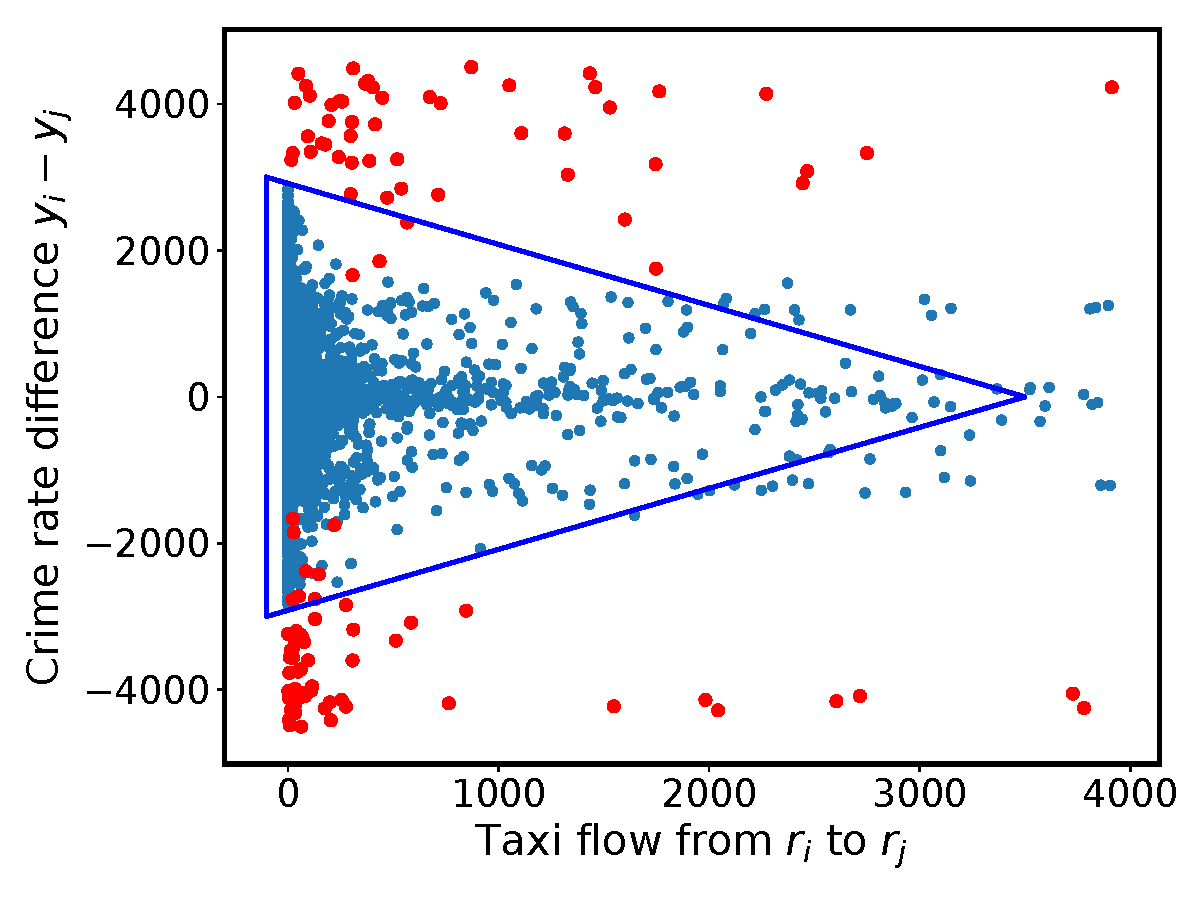
\includegraphics[width=0.6\linewidth]{fig/crime-flow-preliminary.pdf}
\vspace{-3mm}
\caption{The crime rate difference vs. traffic flow volumes for every pair of regions $\langle r_i, r_j \rangle$. Points forming the blue triangle shape indicate that the larger the flow between region $r_i$ and region $r_j$ is, the difference between their crime rates is smaller. The red point denotes a pair of regions with one region being the downtown area.}
\label{fig:prelm}
\end{figure}

Overall, the blue points in Figure~\ref{fig:prelm} validate the intuition of adding taxi flow into prediction model in Equation~(\ref{eq:gim}). However, we notice that there are  many red region pairs do not follow this intuition. The reason is that the downtown region is contained in those pairs. Chicago downtown region has the highest crime rate, and there is a significant amount of traffic between downtown and other regions.

The observation above motivates us to look beyond the traffic volume to determine the relevance measure. As shown in the Figure~\ref{fig:example}, if we account for the structural information of mobility flow, the downtown is a popular hub, which differentiates itself from most of other regions. The graph embedding method is therefore a sound solution to estimate region relevance by modeling such structural information.

